\documentclass[a4paper, 12pt, titlepage]{article}

%
% Importering av pakker
%
\usepackage[latin1]{inputenc}
\usepackage[T1]{fontenc, url}
%\usepackage{babel}
\usepackage{textcomp}
\usepackage{amsmath, amssymb}
\usepackage{amsbsy, amsfonts}
\usepackage{graphicx, color}
\usepackage{parskip}
%
% Parametere for inkludering av kode fra fil
%
\usepackage{listings}
\lstset{language=python}
\lstset{basicstyle=\ttfamily\small}
\lstset{frame=single}
\lstset{keywordstyle=\color{red}\bfseries}
\lstset{commentstyle=\itshape\color{blue}}
\lstset{showspaces=false}
\lstset{showstringspaces=false}
\lstset{showtabs=false}
\lstset{breaklines}

%
% Layout
%
\topmargin = -40pt
\oddsidemargin = -15pt
\textheight = 710pt
\textwidth = 460pt

%
% Definering av egne kommandoer og miljøer
%
\newcommand{\dd}[1]{\ \text{d}#1}
\newcommand{\f}[2]{\frac{#1}{#2}} 
\newcommand{\beq}{\begin{equation*}}
\newcommand{\eeq}{\end{equation*}}
\newcommand{\bt}[1]{\textbf{#1}}
\newcommand{\n}{\newline}
%
% Navn og tittel
%
\author{Fredrik WIlhelm Holmen}
\title{Project 4}
\title{FYS3150}

\begin{document}
  \maketitle
  \newpage
  \begin{section}*{Analytical solution}
    The diffusion equations is given as: \beq \f{\partial u}{\partial t} = D\f{\partial ^2u}{\partial x^2}\eeq
    We want the boundary conditions equal to $0$, so we define a new function \beq v(x,t) = u(x,t) - u_s(x,t) \eeq
    and solve the diffusion equation for this function. This equation can be solved by separation of
    variables. Setting $v(x,t) = X(x)T(t)$ gives:
    \beq \f{dT}{dt} \f{1}{T(t)} \f{1}{D^2} = \f{1}{X(x)} \f{d^2 X}{dx^2}\eeq
    Both LHS and RHS must be equal to the same constant for this equation to hold at all times. We get:
    \beq \f{dT}{dt} \f{1}{T(t)} \f{1}{D^2} = -\lambda ^2 \text{and }\f{1}{X(x)} \f{d^2 X}{dx^2} = -\lambda ^2 \eeq 
    The soltion for the time equation is \beq T(t) = e^{-D^2\lambda ^2 t} \eeq while the spacial solution is
    \beq X(x) = Asin(\lambda x) + Bcos(\lambda x) \eeq
    Setting $ D = 1$.
    By the boundary conditions $v(0,t) = v(1,t) = 0$ we see that $B = 0$ and that $\lambda = n\pi$. 
    So we get \beq v(x,t) = \sum_{n=1}^{\infty} C_n sin(n\pi x) e^{-n^2\pi ^2 t} \eeq
    The initial condition is given on the form $Ax + b$, so $u_s(x) = 1-x$ fullfills the boundary conditions. 
    We have defined $v(x,t) = u(x,t) - u_s(x)$ so $u(x,t) = v(x,t) + u_s(x)$, 
    \beq u(x,t) = 1 - x + \sum_{n=1}^{\infty} C_n sin(n\pi x)e^{-n^2\pi ^2 t}  \eeq 
    
    To find the $C_n$s, I solve the equation for time equal to 0. I know that $u(x,0) = 0$ for $0<x<1$, so
    \beq v(x,0) = \sum_{n=1}^{\infty} C_n sin(n\pi x) = x - 1 \eeq
    Using the fourier expansion we see that \beq C_n = \f{-2}{\pi n} \eeq and we get the full solution
    \beq v(x,t) = \sum_{n=1}^{\infty} \f{-2}{\pi n} sin(n\pi x) e^{-n^2\pi ^2 t} \eeq
    
    Since this should be solved for $u(x,t)$, we get
    \beq u(x,t) = \sum_{n=1}^{\infty} \f{-2}{\pi n} sin(n\pi x) e^{-n^2\pi ^2 t} + x - 1 \eeq
    
  \end{section}
    
  
  
  \begin{section}*{Algorithms}
    I will use three different schemes to solve the diffusion equation. First I have implemented
    the explicit scheme, then the implicit scheme, and at last I will use Crank-Nicolson.
    \par 
    {\bf The explicit scheme} \par
      The Explicit scheme is a very straight-forward coding of the following equation. 
			\beq
			v_{i,j+1} = \alpha v_{i-1,j} + (1-2\alpha)v_{i,j} + \alpha v_{i+1,j}
			\eeq
      where \beq \alpha = \f{\Delta t}{\Delta x^2} \eeq    
      and the error going as \beq O(\Delta t, \Delta x^2) \eeq
      One can see that without boundary and initial conditions, this equation is unsolvable, but
      since we have the conditions given, we do not need to compute for $j=0$ and $i=0$ or $i=j$.
      \beq \text{boundary conditions: } v(0) = v(L) = 0 \eeq 
      
      Since we are solving for $v(x,t)$, we need to use the initial state given from the analytical 
      section above: \beq v(x,0) = x - 1, \text{ for } 0<x<1 \text{ and } v(0,0) = v(1,0) = 0 \eeq
      
    
    {\bf The Implicit scheme} \par
      The implicit scheme is obtained by using the backward formula for the first derivative. This will
      result in the matrix-vector multiplication: \beq Av_j = v_{j-1} \eeq where A is a tridiagonal matrix
      with off-diagonal elements $-\alpha$ and diagonal elements $1+2\alpha$\par
      I solve this equation by using the solver from project 1 by setting $v_0$ by the initial conditions 
      and the boundary conditions. Then I solve the equation $N_t$ times to . \par
    {\bf The Crank-Nicolson scheme}
      The Crank-Nicolson scheme is a combination of the implicit and the explicit schemes. 
      This scheme is shortly written as \beq (2I + \alpha B) V_j = (2I - \alpha B) V_{j-1} \eeq
     
  \end{section}
  \begin{section}*{Numerical Notes}
   When using $\Delta x = \f{1}{10}$ and $\Delta t = \f{1}{100}$, the Explicit scheme will go berzerk and give horrible 
   results. This is because this scheme is unstable for $\Delta t \geq \f{1}{2}\Delta x^2$. So when increasing
   $\Delta t$ to $\Delta t = \f{1}{200}$ I get stable results. 
   
   None of the numerical approximations manage to overlap with the analytical solution, even though 
   Crank-Nicolson is pretty close. The error for Crank-Nicolson is smaller because the error goes as
   $\Delta t^2$ and $\Delta x^2$, but for explicit and implicit scheme, the error goes as $\Delta x^2$
   and $\Delta t^2$.
  \end{section}

  \begin{section}*{Results and plots}
    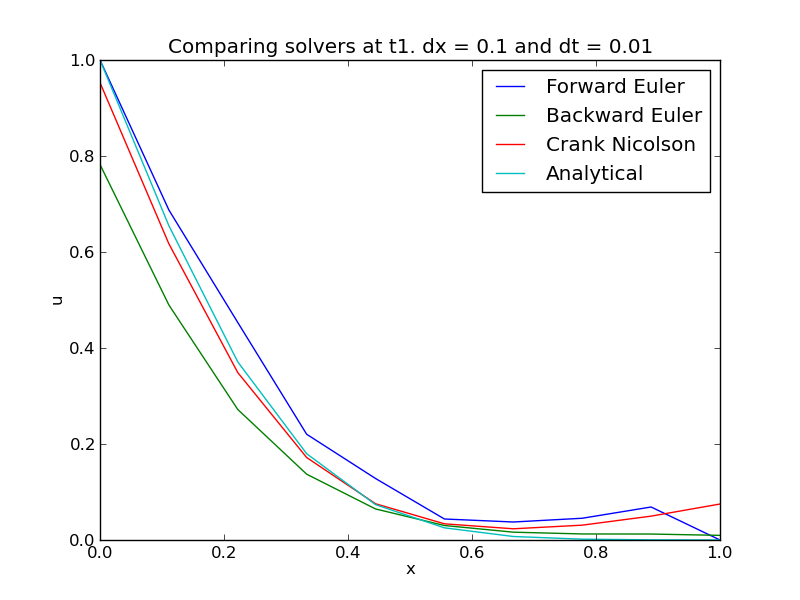
\includegraphics[width=1\textwidth]{build-project4-Desktop-Debug/solverst1.png}
    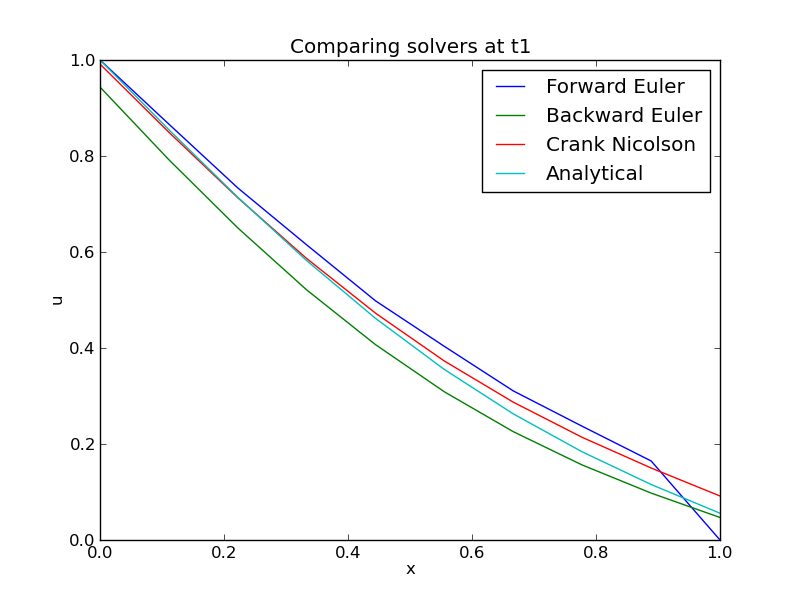
\includegraphics[width=1\textwidth]{build-project4-Desktop-Debug/solverst2.png}
    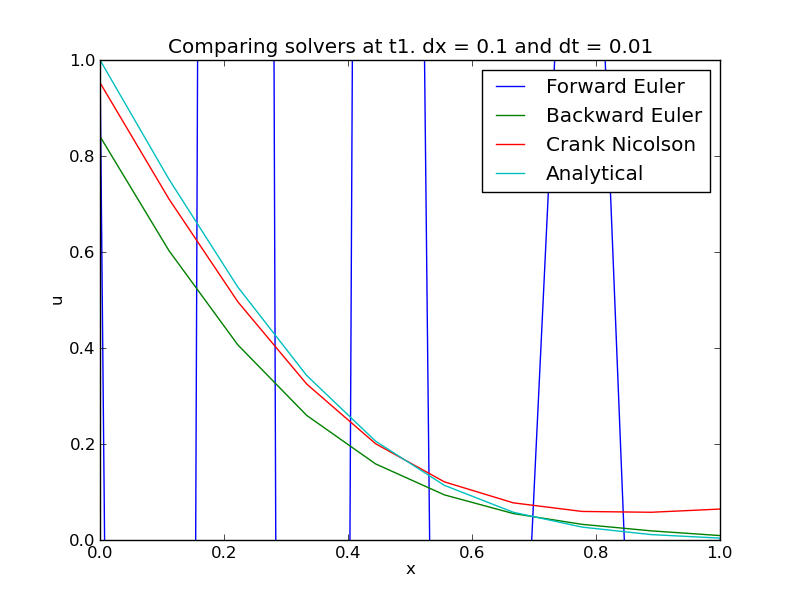
\includegraphics[width=1\textwidth]{build-project4-Desktop-Debug/solverst1_crash.png}
  \end{section}

  
\end{document}